\documentclass[Rapport]{subfiles}
\begin{document}

\chapter{Resultat}
\label{sec:Resultat}

% Inledande text?

Det föregånde kapitlet beskrev hur optimeringen sker via optimise.
I det här avsnittet beskrivs hur kod ser ut efter optimering, och 
olika körningar med och utan optimise jämförs. 
Vi testar endast CBN-semantiken med anropsstack då det är projektets 
slutgiltiga och mest förfinade optimeringsvariant.

Det finns massor av platser i kod där optimise kan placeras, men alla dessa är tyvärr 
inte bra val. Det finns flera fallgropar att undvika för få ut så stor 
prestandavinst som möjligt. Vi ska illusterara detta igenom att undersöka ett 
några större exempel, bland annat en raytracer.

\paragraph{Hur testerna har gjorts}
För att utföra dessa test, har vi använt Haskellbiblioteket Criterion\footnote{http://hackage.haskell.org/package/criterion}.
Varje testprogram som skall testas kommer Criterion att köra 100 gånger. Skräpsamlaren
aktiveras mellan körningarna för att undvika störningar.
En annan detalj är att Criterion 
rapporterar inom vilket konfidensintervall det går att lita
på den uppmätta tiden genom att
mäta störningar (andra program som körs
i bakgrunden et.c.).


\section{Raytracer}


En raytracer är ett program som målar upp en bild genom att skicka ut strålar från en punkt
i ett rum och sedan se vad varje stråle träffar\footnote{Likt hur 
våra egna ögon fungerar. Fast vi skickar inte ut strålar.}.
Utifrån detta kan den sedan bygga upp en bild. Vi har implementerat
en mycket enkel sådan, där rummet består av en djupsorterad lista av tvådimensionella objekt.
Varje objekt beskrivs av en funktion, $Punkt \mapsto Bool$, där den booleska
variabeln svarar på frågan ``Ligger den här punkten inom objektet?''.

För att underlätta ges de tänkta typerna för funktionerna som kommentarer ovanför definitionerna.
En cirkel med radie \ic{1.0} och en kvadrat med sidorna \ic{2.0} defineras:

\begin{codeEx}
-- type Shape = Pos -> Bool
-- circle, square :: Shape

circle p = case p of
    { Pos x y -> x *. x + y *. y <. 1.0
    };

square p = case p of
    { Pos x y -> x >. -1.0 && x <. 1.0
              && y >. -1.0 && y <. 1.0
    };
\end{codeEx}

Vi har sedan en rad kombinatorer för att bygga upp mer komplexa objekt:
translation, skalning, rotation, och olika sätt att sammanfoga flera objekt.

\begin{codeEx}
-- translate, scale :: Pos -> Shape -> Shape
translate dp s p = s $ posSub p dp;
scale     dp s p = s $ posDiv p dp;

-- rotate :: Double -> Shape -> Shape
rotate theta s p = s (polar (abs' p) (arg p +. theta));

-- union, minus, intersect :: Shape -> Shape -> Shape
union     s t p = s p || t p;
minus     s t p = s p && not (t p);
intersect s t p = s p && t p;
\end{codeEx}

Vi ser att ett komplext objekt bara blir en sammasättning av booleska 
funktioner, vilket vid optimering kan infogas och till slut bli ett enda stort \kw{case}-träd. 
Låt oss börja med att betrakta en enkel figur, en fyrkant med sina sidor
nerskalade till 1.0.

\begin{codeEx}
box  = scale (Pos 0.5 0.5) square;
box' = optimise box;
\end{codeEx}

\ic{box} är en partiellt applicerad funktion från \kw{Pos} till \kw{Bool} och
är intressant att optimera: bland annat kommer funktionsanrop att infogas
och onödiga \obj{THUNK}-objekt elimineras.
Såhär ser den optimerade boxfunktionen ut i STG-kod. För att förenkla läsningen har vi tagit bort aktiveringspostindex från variablerna i följande kod:
%Den är lite svår att tyda 
%eftersom alla aktiveringspostindex står med:

\begin{codeEx}
  box' = FUN (p -> case p of
     { Pos x1 y1 -> let
         { a = THUNK (i.bu x1 i.bw)
         } in let
           { b = THUNK (i.bu y1 i.bx)
           } in let
             { c = THUNK  (let
                 { d = THUNK (let
                     { tempOne = CON (D# 1.0)
                     } in a <. tempOne)
                 } in let
                   { e = THUNK (let
                       { f = THUNK (let
                           { tempNegOne = CON (D# -1.0)
                           } in d >. tempNegOne)
                       } in let
                         { g = THUNK (let
                             { tempOne' = CON (D# 1.0)
                             } in f <. tempOne')
                         } in and e g)
                   } in and d e)
             } in case x1 of
               { D# h -> case h /.# 0.5 of
                   { i -> case i >.# -1.0 of
                       { j -> case j of
                           { True  -> c
                           ; False  -> False
                           }
                       }
                   }
               }
     })
\end{codeEx}


Denna version av koden är billig att få fram ur tidssynpunkt och ger ganska
mycket snabbare kod som vi ska se i nästa underavsnitt. Om vi använder 
\kw{casebranches} på samma exempel fås ännu finare kod som bara består av en
rad med \kw{case}-satser, men optimeringen tar mycket längre tid:

\begin{codeEx}
box' = FUN (p -> case p of
   { Pos x1 y1 -> case x1 of
      { D# x1' -> case x1' /.# 0.5 of
         { a -> case a >.# -1.0 of
            { b -> case b of
               { True  -> case a <.# 1.0 of
                  { c -> case c of
                     { True  -> case y1 of
                        { D# y' -> case y' /.# 0.5 of
                           { d -> case d >.# -1.0 of
                              { e -> case e of
                                 { True  -> case d <.# 1.0 of
                                    { f -> f
                                    }
                                 ; False  -> False
                                 }
                              }
                           }
                        }
                     ; False  -> False
                     }
                  }
               ; False  -> False
               }
            }
         }
      }
   })
\end{codeEx}


Så länge endast en färg, förutom bakgrundsfärgen, används kan alla tänkbara figurer modelleras
med objekt i denna implementation. Om det finns intresse för olika färger krävs det
flera objekt. Vi har valt att se varje objekt som ett par
av en färg och en funktion som säger om en punkt ligger innanför objektets ramar. 
Alla sådana par placeras i en lista där första elementet är det
objekt som ska målas upp närmast betraktaren. 

Funktionen \ic{shapes} tar en sådan lista av par av färger och funktioner och 
ger tillbaka en ny funktion från punkt till färg. Den funktionen kan
appliceras på alla punkter för att skapa en bild. I exemplet nedan används \ic{screen}
för att generera alla punkter givet storleken i x- och y-led. I \ic{pic} skapas 
bilden genom att använda \ic{map} med funktionen som fås av \ic{shapes}.

\begin{codeEx}

-- screen :: Double -> Double -> [[Pos]]
screen szX szY = let { xs = fromTo -1.0 (2.0 /. (szX -. 1.0)) 1.0
                     ; ys = fromTo -1.0 (2.0 /. (szY -. 1.0)) 1.0
                     }
                 in map (\x . map (\y . Pos x y) ys) xs;

pic = map (map (shapes [Tuple box red])) (screen x y);

\end{codeEx}

Om man nu vill optimera ovanstående finns det ett par olika tillvägagångssätt. 
Det som har varit mest effektivt när vi testat är att optimera varje objekt för sig. 
Det är även så vi gör i våra testresultat, fast för en mer avancerad scen, t.ex: 
\begin{codeEx}
map (map (shapes 
             [ Tuple (optimise box) red
             , Tuple (optimise sky) blue 
             ])
         )) (screen x y);
\end{codeEx}


\paragraph{Körningstider}

Nu ska vi se hur körningstiden påverkas i ett lite större exempel som består av
en lista med olika figurer som i exemplet ovan. Figur \ref{fig:Resultat:shapes:bild} visar hur
resultatbilden ser ut, bestående av cirklar och kvadrater som är transformerade på olika sätt:

\begin{figure}[H]
\centering
    
\includegraphics[width=0.3\textwidth]{img/shapes.png}
    \caption{Testprogrammets resultat}
    \label{fig:Resultat:shapes:bild}
\end{figure}

Detta program körs sedan på olika stora upplösningar, med och utan optimise,
samt med optimise och casebranchoptimeringen. Hur de två olika
optimeringsvarianterna presterar relativt utan optimering ses i 
den normerade grafen, figur \ref{fig:Resultat:shapes:normgraf}.

\begin{figure}[H]
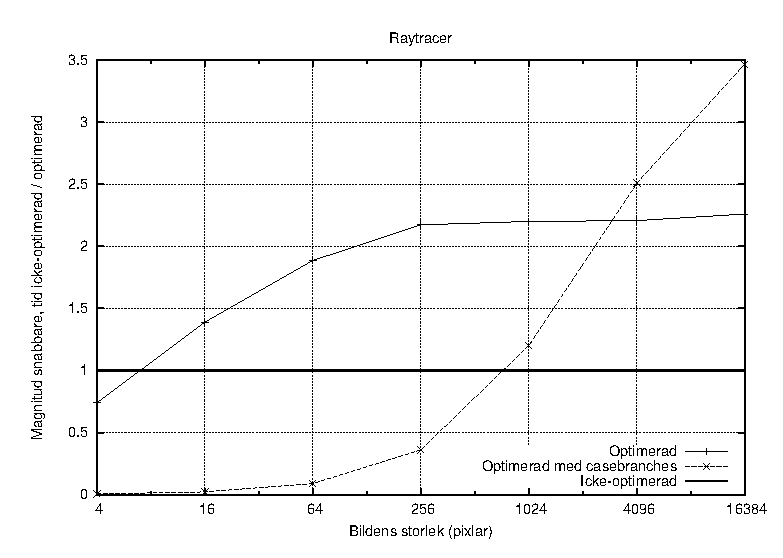
\includegraphics{shapesnorm.eps}
\caption{Normerad tid över körningstiden för raytracern, med och utan
casebranchoptmering, normerat mot utan optimeringen}
\label{fig:Resultat:shapes:normgraf}
\end{figure}

\begin{comment}
Här är vi inte så konsekventa med casebranches och casebraches-optimeringen
och det står typ tre gånger i varje mening
\end{comment}

I den normerade grafen, figuren ovan, ses
på x-axeln bildens storlek i pixlar i logaritmisk skala
på y-axeln ses antalet gånger snabbare de två olika optimeringsmetoderna är relativt
utan optimering. 
För mycket små bilder tar det mer tid att optimera än att bara köra
funktionen för dessa enstaka pixlar. Utan \kw{casebranches} stabiliseras
snabbheten för bilder med många pixlar, 256 och uppåt, till att vara lite över dubbelt
så snabb.
Med \kw{casebranch}-optimeringen tar det initialt mycket lång tid, men funktionen blir
så mycket snabbare att det för stora bilder går det avsevärt mycket snabbare, med 
en faktor större än tre.

Den optimerade funktionen utan \kw{casebranches} är två magnituder snabbare
än med \kw{casebranches} för mycket små bilder. Detta är för att optimise
lägger ner mer tid på \kw{casebranch}-optimeringen.
För stora bilder vinner man ändå på att använda \kw{casebranches}, eftersom optimeringstiden
också här ändå bara är konstant. Vid körning av den optimerade funktionen
behöver inga uppslag i heapen eller icke-primitiva funktionsanrop utföras. 
Troligen kommer den också att plana
ut och bli en konstant gånger snabbare än utan optimering. Då det tar
lång tid\footnote{ 24h eller mer} att köra för stora bilder
har inga sådana test gjorts.


            \begin{comment}
            Körningstiderna visas i figur \ref{fig:Resultat:shapes:loggraf}, som även visar
            hur \kw{casebranches} påverkar resultatet:

            \begin{figure}[H]
            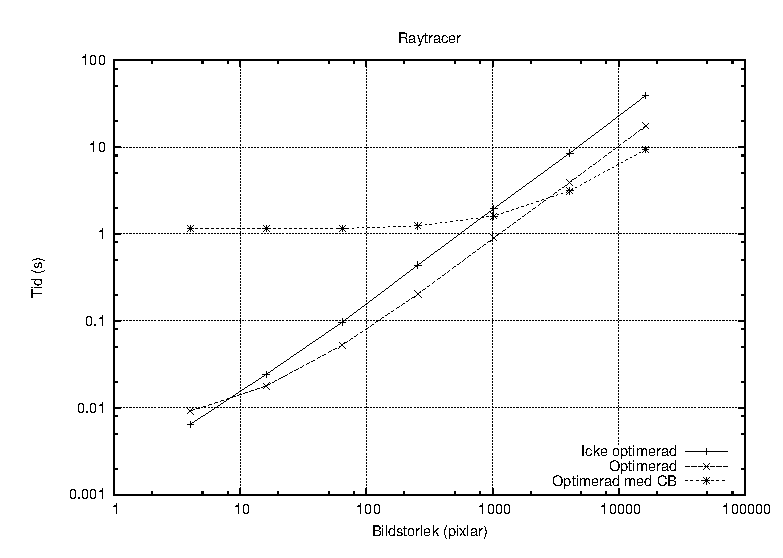
\includegraphics{shapes.eps}
            \caption{Logaritmisk graf över körningstid för raytrace, med och utan optimise.}
            \label{fig:Resultat:shapes:loggraf}
            \end{figure}
            \end{comment}

\section{Powerfunktionen}
Nästa exempel kommer från den välkända \ic{power}-funktionen där vi upphöjer varje element i en lista med tal till ett givet heltal. Funktionen testas med följande kod:
\begin{codeEx}
main = map (optimise (power getInt)) getIntList;

power to x = case to == 0 of
    { True  -> 1
    ; False -> x * power (to - 1) x
    };
\end{codeEx}

Låter vi \ic{getInt} $\mapsto 4$ kommer följande kod att generas vid optimering.

\begin{codeEx}
power_4 = FUN (x -> case x of
    { I# x' -> case x' *# 1 of
       { a -> case x' *# a of
          { b -> case x' *# b of
             { c -> case x' *# c of
                { d -> let
                   { r = CON (I# d)
                   } in r
                }
             }
          }
       }
    })
\end{codeEx}

Notera hur mönstermatchning endast utförs en gång på \ic{x}, och hur det bara
finns primitiva funktionsanrop kvar samt endast en boxning. 

\kw{casebranches}-inställningen gör här ingen skillnad. 
Anledningen till detta är att det bara finns en gren till varje \kw{case}-sats
och då optimeras grenen ändå alltid, 
eftersom inget brott mot semantiken hos STG kan ske.

\paragraph{Körningstider}

Figur \ref{fig:Resultat:power:graf} visar den normerade grafen för körningstid
med optimise för programmet ovan, för olika värden på \ic{getInt}, exponenten. 
\ic{getIntList} är en lista innehållande talen mellan $1 \ldots 200$, storleken på
denna lista är således konstant för alla test.

\begin{figure}[H]
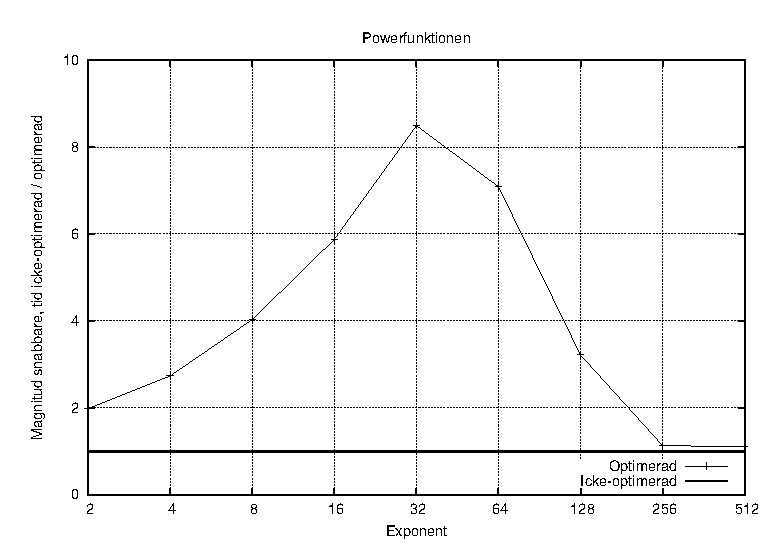
\includegraphics{powernorm.eps}
\caption{Normerad graf över körningstid för power med känd exponent.}
\label{fig:Resultat:power:graf}
\end{figure}

För låga exponenter tar inte optimeringen särskilt mycket tid och
den ger en rejäl tidsvinst - upp mot åtta gånger snabbare.
Vid exponenter högre än 32 tar optimeringen så lång tid att tidsvinsten
blir mindre och efter 256 planar det ut och blir endast marginellt snabbare.
Detta beteende diskuteras i sektion \ref{sec:diskussion_om_exponentialitet}.

                \begin{comment}
                \begin{figure}[H]
                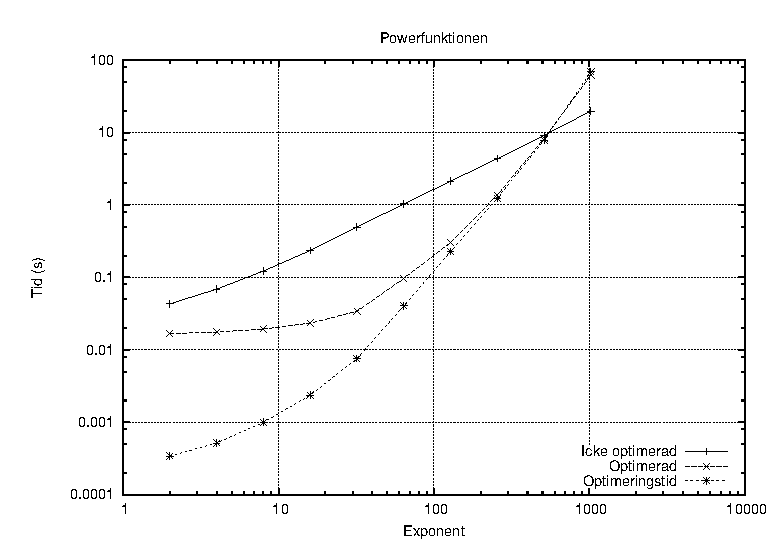
\includegraphics{power.eps}
                \caption{Logaritmisk graf över körningstid för power med känd exponent.
                Med och utan optimise.}
                \label{fig:Resultat:shapes:graf}
                \end{figure}
                \end{comment}

\section{Reguljäruttryck}

Reguljäruttryck är ett sätt att beskriva struktur hos strängar, eller vilka
listor av symboler som helst. Dessa byggs upp av bokstäver
(\ic{a},\ic{b},\ic{c} osv), 
kan konkateneras (med \ic{.}) 
, alterneras (med \ic{|})
 och upprepas (med \ic{*}). 
Som exempel matchar reguljäruttrycket \ic{a.b.c} endast strängen \ic{``abc''},
men \ic{(a|b)*} matchar vilken sträng som helst som består av noll eller fler
\ic{a} eller \ic{b}. Jämför den sista med \ic{(a*)|(b*)} som istället accepterar
en sträng av godtyckligt många \ic{a} eller godtyckligt många \ic{b}, men inte 
en blandning av dem.

Optimeringsfunktionaliteten har testats på ett program som parsar ett reguljäruttryck
och sen en sträng och avgör huruvida den matchar uttrycket. Att optimera 
matchingsfunktionen, \ic{match :: RegExp -> String -> Bool}, med det givna
reguljäruttrycket har undersökts. Resultatet är att det tar ungefär samma
tid med och utan optimeringen. 

Skälet till detta är att då funktionen \ic{match} optimeras infogas
vissa funktionsanrop. I koden för match kommer nya anrop till \ic{match}.
Förvisso kan dessa infogas, men de infogningar kommer att ske så länge som det
finns sträng kvar. Men under optimeringen är den okänd och kan således betraktas
som potentiellt oändlig! Det som skulle ha varit ett intressant beteende var
om anropet till \ic{match} kunde bytas ut till ett anrop till funktionen
som optimeras. Detta diskuteras mer i sektion
\ref{sec:future-regexp}.



\section{Heapstorlek}
Syftet med detta projekt är förvisso att få program att bli snabbare, men det finns även andra faktorer som är intressanta, som exempelvis hur mycket minne ett program tar med och utan \kw{optimise}. Ett sätt att mäta minnet är att räkna antalet objekt som har allokerats på heapen. Detta är ett lite klumpigt mått då exempelvis objektet \ic{I\# 1} kommer att ha lika stor inverkan som en funktion, men det ger ändå en fingervisning om minnesanvändningen.
Återgår vi till två av de tidigare exemplen, powerfunktionen och raytracern, och plottar deras heapanvänding fås följande figur:

\begin{figure}[H]
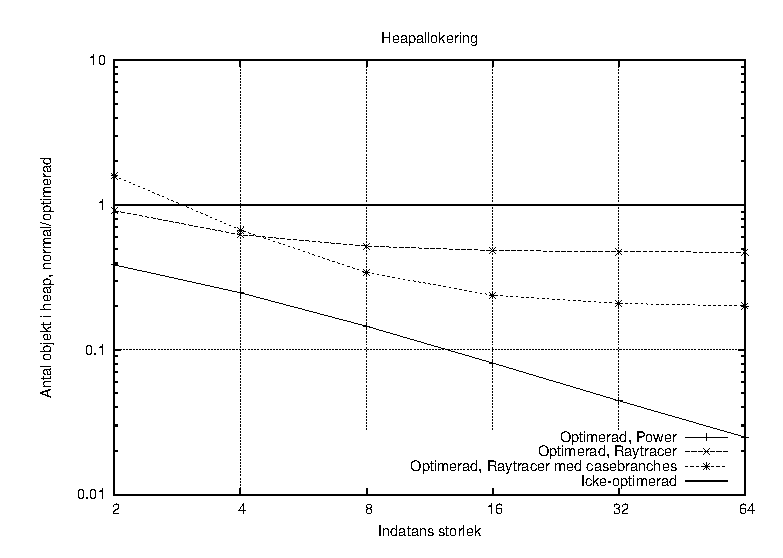
\includegraphics{heap.eps}
\caption{Normerad graf över Heapens storlek}
\label{fig:Resultat:heap:graf}
\end{figure}

I grafen, som är normerad med de icke-optimerade körningarna, ses
på x-axeln indatans storlek (bildytans sida för raytracern och exponenten i power) som ökar logaritmiskt, och 
på y-axeln antalet gånger fler heapobjekt som allokeras med optimering jämfört med utan optimering.
Figuren visar tydligt att antalet heapobjekt som allokeras minskar vid användandet av en optimerad funktion. Detta beror till stor del på att boxade tal inte längre boxas och avboxas för varje primitiv operation, vilka istället är infogade så att avboxningen bara behöver utföras en gång före flera primitiva operationer körs.

Ett vettigt runtimesystem hade naturligtvis skräpsamlat onödiga heapobjekt. För att få ett mått med det inräknat mäts det högsta antalet heapobjekt under körningar med skräpsamling påslagen.
Skräpsamlaren körs mellan varje regel, vilket tar lång tid och gör det praktiskt omöjligt att utföra några större mätningar, men vi har ändå försökt på powerexemplet:

\begin{figure}[H]
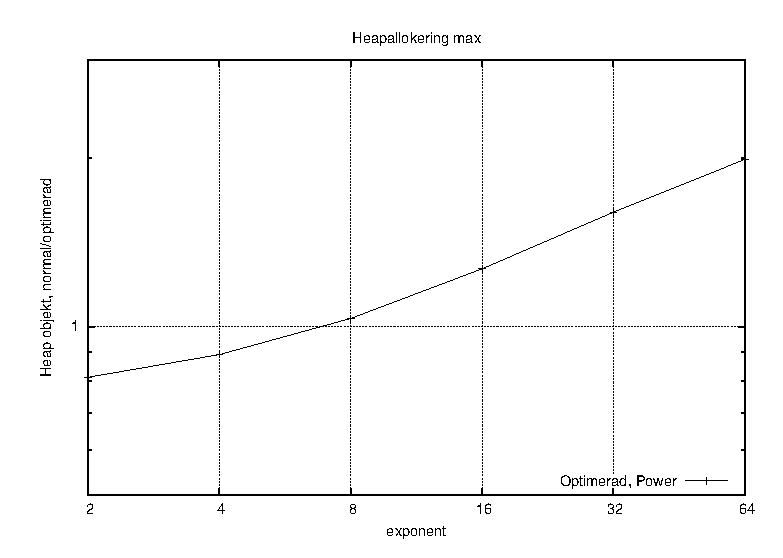
\includegraphics{maxheap.eps}
\caption{Normerad graf över maximala heapstorleken med skräpsamling}
\label{fig:Resultat:maxheap:graf}
\end{figure}

Vi ser att optimerade program för större indata har ett högre maximalt antal objekt i heapen än sina icke-optimerade motsvarigheter. Detta beror på att objekten som allokeras på abyssen hålls aktiva eftersom 
de refereras till av \cont{Olet}-continuations. Detta görs även då de inte kommer att användas, när dödkodseliminering
ändå kommer att ta bort dem. Då denna inverkan inte blir så stor vid små värden på indatan
betyder det att optimeringen till och med gör så att det blir ett mindre antal objekt allokerade än utan i de fallen.


En bra skräpsamlare körs bara ibland och hade därmed inte tagit onödigt lång tid som i testet ovan, men detta skulle ha gjort resultaten från dessa tester osäkrare. \footnote{Dessutom är uppslagnings- och insättningstiden i tolkens heap logaritmisk, vilket kan 
förbättras till konstant tid genom att använda pekare.}











% Kanske borde förklaras bättre. Varför är den inte linjär? :(

\begin{comment}
    \subsection{Expertis}
    Optimise är bra på:
    \begin{itemize}
        \item infogning av funktioner och primitiver
        \item optimera casebranches
        \item beräkna konstantuttryck i en PAP och klistra in resultatet
                 ( detta kan också lösas med full laziness i vissa fall - (vilka?))
    \end{itemize}

    \subsection{Noteringar}

    \NOTE{ 

    \begin{itemize}
        \item Jämför hur kod ser ut före och efter optimering. Förklara lite vad som har gjorts.
            \begin{itemize}
                \item Power har använts som löpande exempel, så vi skulle kunna visa det
                      här också.
                \item Andra program. Förslagsvis något av de lite större exempelprogrammen om vi
                       får dem att fungera bra och kan presentera det på ett vettigt sätt.
                        Shapes, regexp
            \end{itemize}
        \item Jämför snabbheten hos program med och utan optimering (benchmarks)
            \begin{itemize}
                \item Med och utan callstack för att visa hur mycket snabbare resultat det gav oss?
                \item scatterplot för en större mängd program (el. körningar)
        \item Tester med olika stora indata,
            tex listlängd pa x-axeln,
                procentuell ökning på y-axeln,
                upphöjttill-inten på z-axeln.
            
        Antagligen tillräckligt  intressant att ha 2 st av dem, tex optfunktionens storlek mot tid
                                          samt inputens storlek mot tid.
            \end{itemize}
        \item Jämför kodstorlek, komplexitet hos optimise
        \item Hur stor del av tiden går åt till att köra optimise? En graf skulle kunna visa
          detta på ena axeln och listlängd på andra axeln, för att illustrera att
          en optimerad funktion måste köras många gånger för att man ska vinna något på det.

                                          


    \end{itemize}

    }
\end{comment}

% We would be giants, in a land with 
% plentiful of coffee and obviously correct code

\end{document}

